\documentclass[1p]{elsarticle_modified}
%\bibliographystyle{elsarticle-num}

%\usepackage[colorlinks]{hyperref}
%\usepackage{abbrmath_seonhwa} %\Abb, \Ascr, \Acal ,\Abf, \Afrak
\usepackage{amsfonts}
\usepackage{amssymb}
\usepackage{amsmath}
\usepackage{amsthm}
\usepackage{scalefnt}
\usepackage{amsbsy}
\usepackage{kotex}
\usepackage{caption}
\usepackage{subfig}
\usepackage{color}
\usepackage{graphicx}
\usepackage{xcolor} %% white, black, red, green, blue, cyan, magenta, yellow
\usepackage{float}
\usepackage{setspace}
\usepackage{hyperref}

\usepackage{tikz}
\usetikzlibrary{arrows}

\usepackage{multirow}
\usepackage{array} % fixed length table
\usepackage{hhline}

%%%%%%%%%%%%%%%%%%%%%
\makeatletter
\renewcommand*\env@matrix[1][\arraystretch]{%
	\edef\arraystretch{#1}%
	\hskip -\arraycolsep
	\let\@ifnextchar\new@ifnextchar
	\array{*\c@MaxMatrixCols c}}
\makeatother %https://tex.stackexchange.com/questions/14071/how-can-i-increase-the-line-spacing-in-a-matrix
%%%%%%%%%%%%%%%

\usepackage[normalem]{ulem}

\newcommand{\msout}[1]{\ifmmode\text{\sout{\ensuremath{#1}}}\else\sout{#1}\fi}
%SOURCE: \msout is \stkout macro in https://tex.stackexchange.com/questions/20609/strikeout-in-math-mode

\newcommand{\cancel}[1]{
	\ifmmode
	{\color{red}\msout{#1}}
	\else
	{\color{red}\sout{#1}}
	\fi
}

\newcommand{\add}[1]{
	{\color{blue}\uwave{#1}}
}

\newcommand{\replace}[2]{
	\ifmmode
	{\color{red}\msout{#1}}{\color{blue}\uwave{#2}}
	\else
	{\color{red}\sout{#1}}{\color{blue}\uwave{#2}}
	\fi
}

\newcommand{\Sol}{\mathcal{S}} %segment
\newcommand{\D}{D} %diagram
\newcommand{\A}{\mathcal{A}} %arc


%%%%%%%%%%%%%%%%%%%%%%%%%%%%%5 test

\def\sl{\operatorname{\textup{SL}}(2,\Cbb)}
\def\psl{\operatorname{\textup{PSL}}(2,\Cbb)}
\def\quan{\mkern 1mu \triangleright \mkern 1mu}

\theoremstyle{definition}
\newtheorem{thm}{Theorem}[section]
\newtheorem{prop}[thm]{Proposition}
\newtheorem{lem}[thm]{Lemma}
\newtheorem{ques}[thm]{Question}
\newtheorem{cor}[thm]{Corollary}
\newtheorem{defn}[thm]{Definition}
\newtheorem{exam}[thm]{Example}
\newtheorem{rmk}[thm]{Remark}
\newtheorem{alg}[thm]{Algorithm}

\newcommand{\I}{\sqrt{-1}}
\begin{document}

%\begin{frontmatter}
%
%\title{Boundary parabolic representations of knots up to 8 crossings}
%
%%% Group authors per affiliation:
%\author{Yunhi Cho} 
%\address{Department of Mathematics, University of Seoul, Seoul, Korea}
%\ead{yhcho@uos.ac.kr}
%
%
%\author{Seonhwa Kim} %\fnref{s_kim}}
%\address{Center for Geometry and Physics, Institute for Basic Science, Pohang, 37673, Korea}
%\ead{ryeona17@ibs.re.kr}
%
%\author{Hyuk Kim}
%\address{Department of Mathematical Sciences, Seoul National University, Seoul 08826, Korea}
%\ead{hyukkim@snu.ac.kr}
%
%\author{Seokbeom Yoon}
%\address{Department of Mathematical Sciences, Seoul National University, Seoul, 08826,  Korea}
%\ead{sbyoon15@snu.ac.kr}
%
%\begin{abstract}
%We find all boundary parabolic representation of knots up to 8 crossings.
%
%\end{abstract}
%\begin{keyword}
%    \MSC[2010] 57M25 
%\end{keyword}
%
%\end{frontmatter}

%\linenumbers
%\tableofcontents
%
\newcommand\colored[1]{\textcolor{white}{\rule[-0.35ex]{0.8em}{1.4ex}}\kern-0.8em\color{red} #1}%
%\newcommand\colored[1]{\textcolor{white}{ #1}\kern-2.17ex	\textcolor{white}{ #1}\kern-1.81ex	\textcolor{white}{ #1}\kern-2.15ex\color{red}#1	}

{\Large $\underline{12n_{0778}~(K12n_{0778})}$}

\setlength{\tabcolsep}{10pt}
\renewcommand{\arraystretch}{1.6}
\vspace{1cm}\begin{tabular}{m{100pt}>{\centering\arraybackslash}m{274pt}}
\multirow{5}{120pt}{
	\centering
	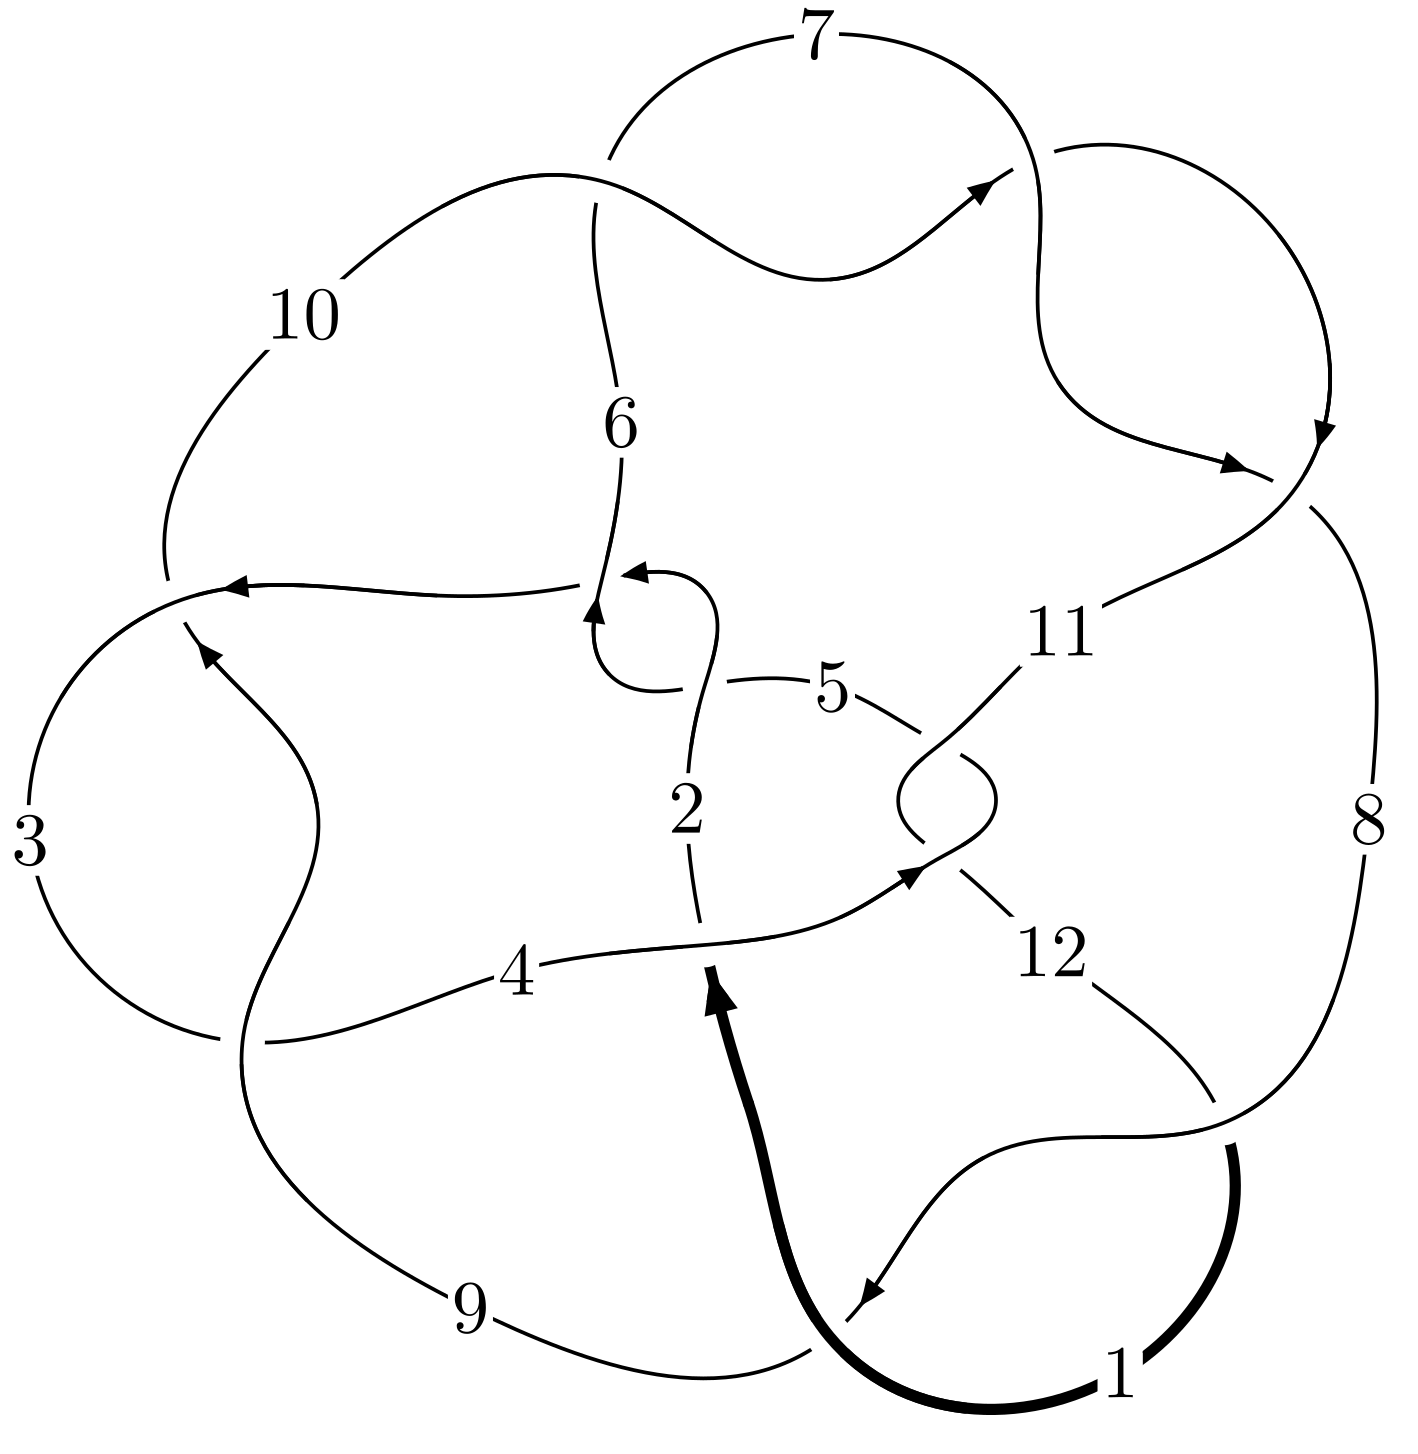
\includegraphics[width=112pt]{../../../GIT/diagram.site/Diagrams/png/2867_12n_0778.png}\\
\ \ \ A knot diagram\footnotemark}&
\allowdisplaybreaks
\textbf{Linearized knot diagam} \\
\cline{2-2}
 &
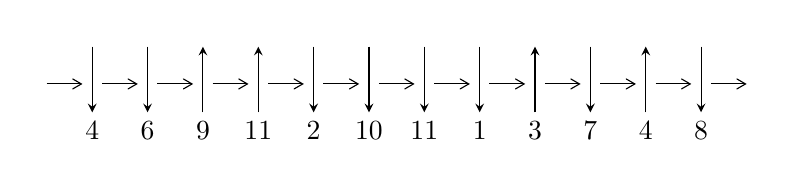
\begin{tikzpicture}[x=20pt, y=17pt]
	% nodes
	\node (C0) at (0, 0) {};
	\node (C1) at (1, 0) {};
	\node (C1U) at (1, +1) {};
	\node (C1D) at (1, -1) {4};

	\node (C2) at (2, 0) {};
	\node (C2U) at (2, +1) {};
	\node (C2D) at (2, -1) {6};

	\node (C3) at (3, 0) {};
	\node (C3U) at (3, +1) {};
	\node (C3D) at (3, -1) {9};

	\node (C4) at (4, 0) {};
	\node (C4U) at (4, +1) {};
	\node (C4D) at (4, -1) {11};

	\node (C5) at (5, 0) {};
	\node (C5U) at (5, +1) {};
	\node (C5D) at (5, -1) {2};

	\node (C6) at (6, 0) {};
	\node (C6U) at (6, +1) {};
	\node (C6D) at (6, -1) {10};

	\node (C7) at (7, 0) {};
	\node (C7U) at (7, +1) {};
	\node (C7D) at (7, -1) {11};

	\node (C8) at (8, 0) {};
	\node (C8U) at (8, +1) {};
	\node (C8D) at (8, -1) {1};

	\node (C9) at (9, 0) {};
	\node (C9U) at (9, +1) {};
	\node (C9D) at (9, -1) {3};

	\node (C10) at (10, 0) {};
	\node (C10U) at (10, +1) {};
	\node (C10D) at (10, -1) {7};

	\node (C11) at (11, 0) {};
	\node (C11U) at (11, +1) {};
	\node (C11D) at (11, -1) {4};

	\node (C12) at (12, 0) {};
	\node (C12U) at (12, +1) {};
	\node (C12D) at (12, -1) {8};
	\node (C13) at (13, 0) {};

	% arrows
	\draw[->,>={angle 60}]
	(C0) edge (C1) (C1) edge (C2) (C2) edge (C3) (C3) edge (C4) (C4) edge (C5) (C5) edge (C6) (C6) edge (C7) (C7) edge (C8) (C8) edge (C9) (C9) edge (C10) (C10) edge (C11) (C11) edge (C12) (C12) edge (C13) ;	\draw[->,>=stealth]
	(C1U) edge (C1D) (C2U) edge (C2D) (C3D) edge (C3U) (C4D) edge (C4U) (C5U) edge (C5D) (C6U) edge (C6D) (C7U) edge (C7D) (C8U) edge (C8D) (C9D) edge (C9U) (C10U) edge (C10D) (C11D) edge (C11U) (C12U) edge (C12D) ;
	\end{tikzpicture} \\
\hhline{~~} \\& 
\textbf{Solving Sequence} \\ \cline{2-2} 
 &
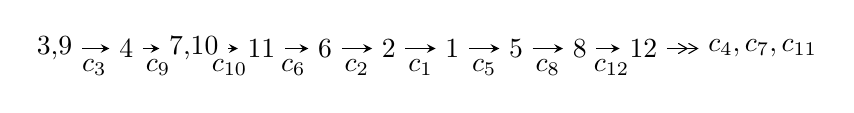
\begin{tikzpicture}[x=23pt, y=7pt]
	% node
	\node (A0) at (-1/8, 0) {3,9};
	\node (A1) at (1, 0) {4};
	\node (A2) at (33/16, 0) {7,10};
	\node (A3) at (25/8, 0) {11};
	\node (A4) at (33/8, 0) {6};
	\node (A5) at (41/8, 0) {2};
	\node (A6) at (49/8, 0) {1};
	\node (A7) at (57/8, 0) {5};
	\node (A8) at (65/8, 0) {8};
	\node (A9) at (73/8, 0) {12};
	\node (C1) at (1/2, -1) {$c_{3}$};
	\node (C2) at (3/2, -1) {$c_{9}$};
	\node (C3) at (21/8, -1) {$c_{10}$};
	\node (C4) at (29/8, -1) {$c_{6}$};
	\node (C5) at (37/8, -1) {$c_{2}$};
	\node (C6) at (45/8, -1) {$c_{1}$};
	\node (C7) at (53/8, -1) {$c_{5}$};
	\node (C8) at (61/8, -1) {$c_{8}$};
	\node (C9) at (69/8, -1) {$c_{12}$};
	\node (A10) at (11, 0) {$c_{4},c_{7},c_{11}$};

	% edge
	\draw[->,>=stealth]	
	(A0) edge (A1) (A1) edge (A2) (A2) edge (A3) (A3) edge (A4) (A4) edge (A5) (A5) edge (A6) (A6) edge (A7) (A7) edge (A8) (A8) edge (A9) ;
	\draw[->>,>={angle 60}]	
	(A9) edge (A10);
\end{tikzpicture} \\ 

\end{tabular} \\

\footnotetext{
The image of knot diagram is generated by the software ``\textbf{Draw programme}" developed by Andrew Bartholomew(\url{http://www.layer8.co.uk/maths/draw/index.htm\#Running-draw}), where we modified some parts for our purpose(\url{https://github.com/CATsTAILs/LinksPainter}).
}\phantom \\ \newline 
\centering \textbf{Ideals for irreducible components\footnotemark of $X_{\text{par}}$} 
 
\begin{align*}
I^u_{1}&=\langle 
2.19719\times10^{90} u^{58}+3.18845\times10^{90} u^{57}+\cdots+8.27618\times10^{90} b+5.36600\times10^{91},\\
\phantom{I^u_{1}}&\phantom{= \langle  }1.26061\times10^{91} u^{58}+1.72237\times10^{91} u^{57}+\cdots+2.48285\times10^{91} a+4.55960\times10^{92},\;u^{59}+u^{58}+\cdots-18 u-9\rangle \\
I^u_{2}&=\langle 
u^{16}- u^{15}+\cdots+5 b-9,\;7 u^{16}+3 u^{15}+\cdots+5 a-28,\;u^{17}+10 u^{15}+\cdots-5 u+1\rangle \\
\\
\end{align*}
\raggedright * 2 irreducible components of $\dim_{\mathbb{C}}=0$, with total 76 representations.\\
\footnotetext{All coefficients of polynomials are rational numbers. But the coefficients are sometimes approximated in decimal forms when there is not enough margin.}
\newpage
\renewcommand{\arraystretch}{1}
\centering \section*{I. $I^u_{1}= \langle 2.20\times10^{90} u^{58}+3.19\times10^{90} u^{57}+\cdots+8.28\times10^{90} b+5.37\times10^{91},\;1.26\times10^{91} u^{58}+1.72\times10^{91} u^{57}+\cdots+2.48\times10^{91} a+4.56\times10^{92},\;u^{59}+u^{58}+\cdots-18 u-9 \rangle$}
\flushleft \textbf{(i) Arc colorings}\\
\begin{tabular}{m{7pt} m{180pt} m{7pt} m{180pt} }
\flushright $a_{3}=$&$\begin{pmatrix}1\\0\end{pmatrix}$ \\
\flushright $a_{9}=$&$\begin{pmatrix}0\\u\end{pmatrix}$ \\
\flushright $a_{4}=$&$\begin{pmatrix}1\\- u^2\end{pmatrix}$ \\
\flushright $a_{7}=$&$\begin{pmatrix}-0.507725 u^{58}-0.693705 u^{57}+\cdots-47.3340 u-18.3644\\-0.265483 u^{58}-0.385257 u^{57}+\cdots-20.1693 u-6.48366\end{pmatrix}$ \\
\flushright $a_{10}=$&$\begin{pmatrix}u\\u\end{pmatrix}$ \\
\flushright $a_{11}=$&$\begin{pmatrix}-1.18361 u^{58}-1.61569 u^{57}+\cdots-147.188 u-26.2949\\0.331778 u^{58}+0.515855 u^{57}+\cdots+42.4239 u+9.96083\end{pmatrix}$ \\
\flushright $a_{6}=$&$\begin{pmatrix}-0.503583 u^{58}-0.697011 u^{57}+\cdots-43.9621 u-17.7685\\-0.261341 u^{58}-0.388563 u^{57}+\cdots-16.7974 u-5.88781\end{pmatrix}$ \\
\flushright $a_{2}=$&$\begin{pmatrix}1.73974 u^{58}+2.35435 u^{57}+\cdots+193.814 u+32.6618\\0.0168231 u^{58}+0.0480879 u^{57}+\cdots-16.3637 u-3.47890\end{pmatrix}$ \\
\flushright $a_{1}=$&$\begin{pmatrix}1.92664 u^{58}+2.62835 u^{57}+\cdots+204.171 u+34.7144\\-0.0640961 u^{58}-0.0778894 u^{57}+\cdots-19.6136 u-4.26282\end{pmatrix}$ \\
\flushright $a_{5}=$&$\begin{pmatrix}1.23803 u^{58}+1.74157 u^{57}+\cdots+163.964 u+31.2786\\-0.729025 u^{58}-0.985396 u^{57}+\cdots-80.2851 u-18.3600\end{pmatrix}$ \\
\flushright $a_{8}=$&$\begin{pmatrix}0.155964 u^{58}+0.116373 u^{57}+\cdots+20.0247 u-5.23157\\-0.846484 u^{58}-1.22210 u^{57}+\cdots-89.6127 u-19.8092\end{pmatrix}$ \\
\flushright $a_{12}=$&$\begin{pmatrix}0.979045 u^{58}+1.35615 u^{57}+\cdots+123.194 u+20.2228\\-0.337866 u^{58}-0.511247 u^{57}+\cdots-39.5933 u-9.46607\end{pmatrix}$\\&\end{tabular}
\flushleft \textbf{(ii) Obstruction class $= -1$}\\~\\
\flushleft \textbf{(iii) Cusp Shapes $= -10.7456 u^{58}-14.9438 u^{57}+\cdots-1129.44 u-248.422$}\\~\\
\newpage\renewcommand{\arraystretch}{1}
\flushleft \textbf{(iv) u-Polynomials at the component}\newline \\
\begin{tabular}{m{50pt}|m{274pt}}
Crossings & \hspace{64pt}u-Polynomials at each crossing \\
\hline $$\begin{aligned}c_{1}\end{aligned}$$&$\begin{aligned}
&u^{59}-6 u^{58}+\cdots-172 u-188
\end{aligned}$\\
\hline $$\begin{aligned}c_{2},c_{5}\end{aligned}$$&$\begin{aligned}
&u^{59}+2 u^{58}+\cdots+16404 u+3277
\end{aligned}$\\
\hline $$\begin{aligned}c_{3},c_{9}\end{aligned}$$&$\begin{aligned}
&u^{59}- u^{58}+\cdots-18 u+9
\end{aligned}$\\
\hline $$\begin{aligned}c_{4},c_{11}\end{aligned}$$&$\begin{aligned}
&u^{59}-3 u^{58}+\cdots-326 u-59
\end{aligned}$\\
\hline $$\begin{aligned}c_{6},c_{7},c_{10}\end{aligned}$$&$\begin{aligned}
&u^{59}+u^{58}+\cdots+55 u-1
\end{aligned}$\\
\hline $$\begin{aligned}c_{8},c_{12}\end{aligned}$$&$\begin{aligned}
&u^{59}-2 u^{58}+\cdots+4 u+19
\end{aligned}$\\
\hline
\end{tabular}\\~\\
\newpage\renewcommand{\arraystretch}{1}
\flushleft \textbf{(v) Riley Polynomials at the component}\newline \\
\begin{tabular}{m{50pt}|m{274pt}}
Crossings & \hspace{64pt}Riley Polynomials at each crossing \\
\hline $$\begin{aligned}c_{1}\end{aligned}$$&$\begin{aligned}
&y^{59}+2 y^{58}+\cdots+493568 y-35344
\end{aligned}$\\
\hline $$\begin{aligned}c_{2},c_{5}\end{aligned}$$&$\begin{aligned}
&y^{59}-44 y^{58}+\cdots+376032834 y-10738729
\end{aligned}$\\
\hline $$\begin{aligned}c_{3},c_{9}\end{aligned}$$&$\begin{aligned}
&y^{59}+61 y^{58}+\cdots+5274 y-81
\end{aligned}$\\
\hline $$\begin{aligned}c_{4},c_{11}\end{aligned}$$&$\begin{aligned}
&y^{59}-35 y^{58}+\cdots+302746 y-3481
\end{aligned}$\\
\hline $$\begin{aligned}c_{6},c_{7},c_{10}\end{aligned}$$&$\begin{aligned}
&y^{59}-59 y^{58}+\cdots+3505 y-1
\end{aligned}$\\
\hline $$\begin{aligned}c_{8},c_{12}\end{aligned}$$&$\begin{aligned}
&y^{59}-24 y^{58}+\cdots+7920 y-361
\end{aligned}$\\
\hline
\end{tabular}\\~\\
\newpage\flushleft \textbf{(vi) Complex Volumes and Cusp Shapes}
$$\begin{array}{c|c|c}  
\text{Solutions to }I^u_{1}& \I (\text{vol} + \sqrt{-1}CS) & \text{Cusp shape}\\
 \hline 
\begin{aligned}
u &= \phantom{-}0.946714 + 0.326161 I \\
a &= \phantom{-}1.56057 - 0.12495 I \\
b &= \phantom{-}0.311162 + 0.580467 I\end{aligned}
 & -1.56439 + 3.00160 I & \phantom{-0.000000 } 0 \\ \hline\begin{aligned}
u &= \phantom{-}0.946714 - 0.326161 I \\
a &= \phantom{-}1.56057 + 0.12495 I \\
b &= \phantom{-}0.311162 - 0.580467 I\end{aligned}
 & -1.56439 - 3.00160 I & \phantom{-0.000000 } 0 \\ \hline\begin{aligned}
u &= \phantom{-}0.274423 + 0.933293 I \\
a &= \phantom{-}1.093080 + 0.183487 I \\
b &= \phantom{-}0.284590 + 0.978686 I\end{aligned}
 & -1.31018 - 2.27927 I & \phantom{-0.000000 } 0 \\ \hline\begin{aligned}
u &= \phantom{-}0.274423 - 0.933293 I \\
a &= \phantom{-}1.093080 - 0.183487 I \\
b &= \phantom{-}0.284590 - 0.978686 I\end{aligned}
 & -1.31018 + 2.27927 I & \phantom{-0.000000 } 0 \\ \hline\begin{aligned}
u &= \phantom{-}0.432068 + 0.950149 I \\
a &= \phantom{-}0.769405 + 0.539694 I \\
b &= \phantom{-}0.959480 + 0.704692 I\end{aligned}
 & \phantom{-}0.84211 - 1.52559 I & \phantom{-0.000000 } 0 \\ \hline\begin{aligned}
u &= \phantom{-}0.432068 - 0.950149 I \\
a &= \phantom{-}0.769405 - 0.539694 I \\
b &= \phantom{-}0.959480 - 0.704692 I\end{aligned}
 & \phantom{-}0.84211 + 1.52559 I & \phantom{-0.000000 } 0 \\ \hline\begin{aligned}
u &= \phantom{-}0.352097 + 0.878149 I \\
a &= -0.045510 - 0.420512 I \\
b &= \phantom{-}0.39071 - 1.47323 I\end{aligned}
 & -3.75832 + 2.49847 I & -12.64369 + 0. I\phantom{ +0.000000I} \\ \hline\begin{aligned}
u &= \phantom{-}0.352097 - 0.878149 I \\
a &= -0.045510 + 0.420512 I \\
b &= \phantom{-}0.39071 + 1.47323 I\end{aligned}
 & -3.75832 - 2.49847 I & -12.64369 + 0. I\phantom{ +0.000000I} \\ \hline\begin{aligned}
u &= -1.13422\phantom{ +0.000000I} \\
a &= -1.26893\phantom{ +0.000000I} \\
b &= -0.0814501\phantom{ +0.000000I}\end{aligned}
 & -6.98624\phantom{ +0.000000I} & \phantom{-0.000000 } 0 \\ \hline\begin{aligned}
u &= \phantom{-}0.561179 + 1.012900 I \\
a &= -0.302808 - 0.673820 I \\
b &= \phantom{-}0.31273 - 1.54903 I\end{aligned}
 & -3.67169 + 2.45859 I & \phantom{-0.000000 } 0\\
 \hline 
 \end{array}$$\newpage$$\begin{array}{c|c|c}  
\text{Solutions to }I^u_{1}& \I (\text{vol} + \sqrt{-1}CS) & \text{Cusp shape}\\
 \hline 
\begin{aligned}
u &= \phantom{-}0.561179 - 1.012900 I \\
a &= -0.302808 + 0.673820 I \\
b &= \phantom{-}0.31273 + 1.54903 I\end{aligned}
 & -3.67169 - 2.45859 I & \phantom{-0.000000 } 0 \\ \hline\begin{aligned}
u &= -1.044970 + 0.554481 I \\
a &= \phantom{-}1.284180 - 0.118622 I \\
b &= \phantom{-}0.348427 - 0.902142 I\end{aligned}
 & -2.53248 - 9.55354 I & \phantom{-0.000000 } 0 \\ \hline\begin{aligned}
u &= -1.044970 - 0.554481 I \\
a &= \phantom{-}1.284180 + 0.118622 I \\
b &= \phantom{-}0.348427 + 0.902142 I\end{aligned}
 & -2.53248 + 9.55354 I & \phantom{-0.000000 } 0 \\ \hline\begin{aligned}
u &= \phantom{-}0.694897 + 0.309169 I \\
a &= -0.655382 - 0.922102 I \\
b &= -0.492656 + 0.163283 I\end{aligned}
 & \phantom{-}2.70885 + 5.61589 I & -3.30287 - 6.43944 I \\ \hline\begin{aligned}
u &= \phantom{-}0.694897 - 0.309169 I \\
a &= -0.655382 + 0.922102 I \\
b &= -0.492656 - 0.163283 I\end{aligned}
 & \phantom{-}2.70885 - 5.61589 I & -3.30287 + 6.43944 I \\ \hline\begin{aligned}
u &= -0.377570 + 1.203860 I \\
a &= \phantom{-}0.551178 - 0.618257 I \\
b &= \phantom{-}0.836117 - 0.754276 I\end{aligned}
 & \phantom{-}0.14649 - 4.50904 I & \phantom{-0.000000 } 0 \\ \hline\begin{aligned}
u &= -0.377570 - 1.203860 I \\
a &= \phantom{-}0.551178 + 0.618257 I \\
b &= \phantom{-}0.836117 + 0.754276 I\end{aligned}
 & \phantom{-}0.14649 + 4.50904 I & \phantom{-0.000000 } 0 \\ \hline\begin{aligned}
u &= -0.727540 + 0.051837 I \\
a &= -0.190027 + 0.786244 I \\
b &= -0.397472 - 0.225985 I\end{aligned}
 & \phantom{-}3.62930 + 0.50765 I & -0.833668 + 0.393936 I \\ \hline\begin{aligned}
u &= -0.727540 - 0.051837 I \\
a &= -0.190027 - 0.786244 I \\
b &= -0.397472 + 0.225985 I\end{aligned}
 & \phantom{-}3.62930 - 0.50765 I & -0.833668 - 0.393936 I \\ \hline\begin{aligned}
u &= -0.219875 + 1.257510 I \\
a &= \phantom{-}0.364413 + 0.342316 I \\
b &= -0.279945 + 0.897413 I\end{aligned}
 & -0.40003 - 2.91377 I & \phantom{-0.000000 } 0\\
 \hline 
 \end{array}$$\newpage$$\begin{array}{c|c|c}  
\text{Solutions to }I^u_{1}& \I (\text{vol} + \sqrt{-1}CS) & \text{Cusp shape}\\
 \hline 
\begin{aligned}
u &= -0.219875 - 1.257510 I \\
a &= \phantom{-}0.364413 - 0.342316 I \\
b &= -0.279945 - 0.897413 I\end{aligned}
 & -0.40003 + 2.91377 I & \phantom{-0.000000 } 0 \\ \hline\begin{aligned}
u &= -1.000700 + 0.859170 I \\
a &= -0.917675 + 0.566007 I \\
b &= -0.110854 + 1.175290 I\end{aligned}
 & -3.32365 + 2.74478 I & \phantom{-0.000000 } 0 \\ \hline\begin{aligned}
u &= -1.000700 - 0.859170 I \\
a &= -0.917675 - 0.566007 I \\
b &= -0.110854 - 1.175290 I\end{aligned}
 & -3.32365 - 2.74478 I & \phantom{-0.000000 } 0 \\ \hline\begin{aligned}
u &= -0.037604 + 1.359730 I \\
a &= \phantom{-}0.67112 - 2.28060 I \\
b &= \phantom{-}0.72572 - 3.32571 I\end{aligned}
 & -4.27309 + 0.18450 I & \phantom{-0.000000 } 0 \\ \hline\begin{aligned}
u &= -0.037604 - 1.359730 I \\
a &= \phantom{-}0.67112 + 2.28060 I \\
b &= \phantom{-}0.72572 + 3.32571 I\end{aligned}
 & -4.27309 - 0.18450 I & \phantom{-0.000000 } 0 \\ \hline\begin{aligned}
u &= -0.225882 + 0.585977 I \\
a &= \phantom{-}0.581173 - 0.021516 I \\
b &= \phantom{-}0.153517 + 0.402501 I\end{aligned}
 & -0.260694 - 1.053330 I & -4.12893 + 6.41098 I \\ \hline\begin{aligned}
u &= -0.225882 - 0.585977 I \\
a &= \phantom{-}0.581173 + 0.021516 I \\
b &= \phantom{-}0.153517 - 0.402501 I\end{aligned}
 & -0.260694 + 1.053330 I & -4.12893 - 6.41098 I \\ \hline\begin{aligned}
u &= \phantom{-}0.122554 + 1.388830 I \\
a &= -0.994864 - 0.157474 I \\
b &= -0.458238 - 0.081576 I\end{aligned}
 & -7.26872 + 1.86522 I & \phantom{-0.000000 } 0 \\ \hline\begin{aligned}
u &= \phantom{-}0.122554 - 1.388830 I \\
a &= -0.994864 + 0.157474 I \\
b &= -0.458238 + 0.081576 I\end{aligned}
 & -7.26872 - 1.86522 I & \phantom{-0.000000 } 0 \\ \hline\begin{aligned}
u &= -0.064719 + 1.399950 I \\
a &= \phantom{-}0.551474 - 0.867993 I \\
b &= -0.18042 - 1.60402 I\end{aligned}
 & -4.84282 - 1.75534 I & \phantom{-0.000000 } 0\\
 \hline 
 \end{array}$$\newpage$$\begin{array}{c|c|c}  
\text{Solutions to }I^u_{1}& \I (\text{vol} + \sqrt{-1}CS) & \text{Cusp shape}\\
 \hline 
\begin{aligned}
u &= -0.064719 - 1.399950 I \\
a &= \phantom{-}0.551474 + 0.867993 I \\
b &= -0.18042 + 1.60402 I\end{aligned}
 & -4.84282 + 1.75534 I & \phantom{-0.000000 } 0 \\ \hline\begin{aligned}
u &= \phantom{-}0.15765 + 1.41350 I \\
a &= -1.30737 + 1.31318 I \\
b &= -1.20152 + 2.27783 I\end{aligned}
 & -11.48850 + 1.95356 I & \phantom{-0.000000 } 0 \\ \hline\begin{aligned}
u &= \phantom{-}0.15765 - 1.41350 I \\
a &= -1.30737 - 1.31318 I \\
b &= -1.20152 - 2.27783 I\end{aligned}
 & -11.48850 - 1.95356 I & \phantom{-0.000000 } 0 \\ \hline\begin{aligned}
u &= -0.20549 + 1.40769 I \\
a &= \phantom{-}0.45179 + 1.89171 I \\
b &= \phantom{-}0.54915 + 3.15852 I\end{aligned}
 & -15.4308 - 2.6517 I & \phantom{-0.000000 } 0 \\ \hline\begin{aligned}
u &= -0.20549 - 1.40769 I \\
a &= \phantom{-}0.45179 - 1.89171 I \\
b &= \phantom{-}0.54915 - 3.15852 I\end{aligned}
 & -15.4308 + 2.6517 I & \phantom{-0.000000 } 0 \\ \hline\begin{aligned}
u &= \phantom{-}0.12784 + 1.44950 I \\
a &= \phantom{-}0.49772 + 2.72782 I \\
b &= \phantom{-}0.51248 + 3.68045 I\end{aligned}
 & -4.61048 + 6.42427 I & \phantom{-0.000000 } 0 \\ \hline\begin{aligned}
u &= \phantom{-}0.12784 - 1.44950 I \\
a &= \phantom{-}0.49772 - 2.72782 I \\
b &= \phantom{-}0.51248 - 3.68045 I\end{aligned}
 & -4.61048 - 6.42427 I & \phantom{-0.000000 } 0 \\ \hline\begin{aligned}
u &= \phantom{-}0.24147 + 1.45902 I \\
a &= \phantom{-}0.195740 - 0.333338 I \\
b &= -0.532485 - 0.754762 I\end{aligned}
 & -3.05183 + 8.97120 I & \phantom{-0.000000 } 0 \\ \hline\begin{aligned}
u &= \phantom{-}0.24147 - 1.45902 I \\
a &= \phantom{-}0.195740 + 0.333338 I \\
b &= -0.532485 + 0.754762 I\end{aligned}
 & -3.05183 - 8.97120 I & \phantom{-0.000000 } 0 \\ \hline\begin{aligned}
u &= -0.513897\phantom{ +0.000000I} \\
a &= \phantom{-}3.15603\phantom{ +0.000000I} \\
b &= -0.176822\phantom{ +0.000000I}\end{aligned}
 & -10.6596\phantom{ +0.000000I} & \phantom{-}6.98370\phantom{ +0.000000I}\\
 \hline 
 \end{array}$$\newpage$$\begin{array}{c|c|c}  
\text{Solutions to }I^u_{1}& \I (\text{vol} + \sqrt{-1}CS) & \text{Cusp shape}\\
 \hline 
\begin{aligned}
u &= \phantom{-}0.35908 + 1.48621 I \\
a &= \phantom{-}0.31558 - 1.94989 I \\
b &= \phantom{-}0.33758 - 3.01668 I\end{aligned}
 & -7.41483 + 7.70510 I & \phantom{-0.000000 } 0 \\ \hline\begin{aligned}
u &= \phantom{-}0.35908 - 1.48621 I \\
a &= \phantom{-}0.31558 + 1.94989 I \\
b &= \phantom{-}0.33758 + 3.01668 I\end{aligned}
 & -7.41483 - 7.70510 I & \phantom{-0.000000 } 0 \\ \hline\begin{aligned}
u &= -0.44114 + 1.47669 I \\
a &= -0.464833 - 1.280610 I \\
b &= -0.53565 - 2.19843 I\end{aligned}
 & -11.91740 - 5.70509 I & \phantom{-0.000000 } 0 \\ \hline\begin{aligned}
u &= -0.44114 - 1.47669 I \\
a &= -0.464833 + 1.280610 I \\
b &= -0.53565 + 2.19843 I\end{aligned}
 & -11.91740 + 5.70509 I & \phantom{-0.000000 } 0 \\ \hline\begin{aligned}
u &= \phantom{-}0.389493 + 0.220844 I \\
a &= -2.44087 + 0.94073 I \\
b &= -0.754459 - 1.051460 I\end{aligned}
 & \phantom{-}0.98362 + 4.60612 I & -4.20164 - 5.47950 I \\ \hline\begin{aligned}
u &= \phantom{-}0.389493 - 0.220844 I \\
a &= -2.44087 - 0.94073 I \\
b &= -0.754459 + 1.051460 I\end{aligned}
 & \phantom{-}0.98362 - 4.60612 I & -4.20164 + 5.47950 I \\ \hline\begin{aligned}
u &= \phantom{-}0.421815\phantom{ +0.000000I} \\
a &= \phantom{-}1.90314\phantom{ +0.000000I} \\
b &= \phantom{-}0.0611523\phantom{ +0.000000I}\end{aligned}
 & -1.31886\phantom{ +0.000000I} & -6.37980\phantom{ +0.000000I} \\ \hline\begin{aligned}
u &= \phantom{-}0.00552 + 1.58194 I \\
a &= -0.499227 - 0.232760 I \\
b &= -0.087958 - 0.208511 I\end{aligned}
 & -7.88129 - 1.40424 I & \phantom{-0.000000 } 0 \\ \hline\begin{aligned}
u &= \phantom{-}0.00552 - 1.58194 I \\
a &= -0.499227 + 0.232760 I \\
b &= -0.087958 + 0.208511 I\end{aligned}
 & -7.88129 + 1.40424 I & \phantom{-0.000000 } 0 \\ \hline\begin{aligned}
u &= \phantom{-}0.404606\phantom{ +0.000000I} \\
a &= \phantom{-}1.10231\phantom{ +0.000000I} \\
b &= \phantom{-}1.14381\phantom{ +0.000000I}\end{aligned}
 & -2.55057\phantom{ +0.000000I} & \phantom{-}7.13820\phantom{ +0.000000I}\\
 \hline 
 \end{array}$$\newpage$$\begin{array}{c|c|c}  
\text{Solutions to }I^u_{1}& \I (\text{vol} + \sqrt{-1}CS) & \text{Cusp shape}\\
 \hline 
\begin{aligned}
u &= \phantom{-}0.12585 + 1.62496 I \\
a &= -0.95051 + 2.36181 I \\
b &= -0.86504 + 3.19856 I\end{aligned}
 & -12.17070 + 4.62001 I & \phantom{-0.000000 } 0 \\ \hline\begin{aligned}
u &= \phantom{-}0.12585 - 1.62496 I \\
a &= -0.95051 - 2.36181 I \\
b &= -0.86504 - 3.19856 I\end{aligned}
 & -12.17070 - 4.62001 I & \phantom{-0.000000 } 0 \\ \hline\begin{aligned}
u &= -0.37010 + 1.59094 I \\
a &= \phantom{-}0.35752 + 2.03746 I \\
b &= \phantom{-}0.31522 + 3.03288 I\end{aligned}
 & -9.4757 - 14.7159 I & \phantom{-0.000000 } 0 \\ \hline\begin{aligned}
u &= -0.37010 - 1.59094 I \\
a &= \phantom{-}0.35752 - 2.03746 I \\
b &= \phantom{-}0.31522 - 3.03288 I\end{aligned}
 & -9.4757 + 14.7159 I & \phantom{-0.000000 } 0 \\ \hline\begin{aligned}
u &= \phantom{-}0.365225\phantom{ +0.000000I} \\
a &= -2.32338\phantom{ +0.000000I} \\
b &= \phantom{-}1.24588\phantom{ +0.000000I}\end{aligned}
 & -6.61235\phantom{ +0.000000I} & -20.0250\phantom{ +0.000000I} \\ \hline\begin{aligned}
u &= -0.17738 + 1.74654 I \\
a &= -0.46710 - 2.03444 I \\
b &= -0.40433 - 2.83686 I\end{aligned}
 & -12.58460 - 1.90611 I & \phantom{-0.000000 } 0 \\ \hline\begin{aligned}
u &= -0.17738 - 1.74654 I \\
a &= -0.46710 + 2.03444 I \\
b &= -0.40433 + 2.83686 I\end{aligned}
 & -12.58460 + 1.90611 I & \phantom{-0.000000 } 0 \\ \hline\begin{aligned}
u &= -0.169630 + 0.056480 I \\
a &= -7.62669 + 0.37534 I \\
b &= -0.832136 - 0.476957 I\end{aligned}
 & \phantom{-}0.101047 - 0.878351 I & -4.40864 + 3.72300 I \\ \hline\begin{aligned}
u &= -0.169630 - 0.056480 I \\
a &= -7.62669 - 0.37534 I \\
b &= -0.832136 + 0.476957 I\end{aligned}
 & \phantom{-}0.101047 + 0.878351 I & -4.40864 - 3.72300 I\\
 \hline 
 \end{array}$$\newpage\newpage\renewcommand{\arraystretch}{1}
\centering \section*{II. $I^u_{2}= \langle u^{16}- u^{15}+\cdots+5 b-9,\;7 u^{16}+3 u^{15}+\cdots+5 a-28,\;u^{17}+10 u^{15}+\cdots-5 u+1 \rangle$}
\flushleft \textbf{(i) Arc colorings}\\
\begin{tabular}{m{7pt} m{180pt} m{7pt} m{180pt} }
\flushright $a_{3}=$&$\begin{pmatrix}1\\0\end{pmatrix}$ \\
\flushright $a_{9}=$&$\begin{pmatrix}0\\u\end{pmatrix}$ \\
\flushright $a_{4}=$&$\begin{pmatrix}1\\- u^2\end{pmatrix}$ \\
\flushright $a_{7}=$&$\begin{pmatrix}-\frac{7}{5} u^{16}-\frac{3}{5} u^{15}+\cdots-\frac{43}{5} u+\frac{28}{5}\\-\frac{1}{5} u^{16}+\frac{1}{5} u^{15}+\cdots-\frac{14}{5} u+\frac{9}{5}\end{pmatrix}$ \\
\flushright $a_{10}=$&$\begin{pmatrix}u\\u\end{pmatrix}$ \\
\flushright $a_{11}=$&$\begin{pmatrix}-\frac{3}{5} u^{16}-\frac{2}{5} u^{15}+\cdots-\frac{12}{5} u+\frac{2}{5}\\u^{10}+u^9+6 u^8+5 u^7+12 u^6+9 u^5+9 u^4+7 u^3+2 u^2+2 u-1\end{pmatrix}$ \\
\flushright $a_{6}=$&$\begin{pmatrix}-\frac{6}{5} u^{16}-\frac{4}{5} u^{15}+\cdots-\frac{29}{5} u+\frac{24}{5}\\u^2+1\end{pmatrix}$ \\
\flushright $a_{2}=$&$\begin{pmatrix}\frac{7}{5} u^{16}+\frac{3}{5} u^{15}+\cdots+\frac{43}{5} u-\frac{23}{5}\\- u^4-2 u^2-1\end{pmatrix}$ \\
\flushright $a_{1}=$&$\begin{pmatrix}\frac{9}{5} u^{16}+\frac{1}{5} u^{15}+\cdots+\frac{51}{5} u-\frac{31}{5}\\\frac{3}{5} u^{16}-\frac{3}{5} u^{15}+\cdots+\frac{12}{5} u-\frac{7}{5}\end{pmatrix}$ \\
\flushright $a_{5}=$&$\begin{pmatrix}\frac{3}{5} u^{16}-\frac{3}{5} u^{15}+\cdots+\frac{22}{5} u-\frac{2}{5}\\- u^6-3 u^4-2 u^2\end{pmatrix}$ \\
\flushright $a_{8}=$&$\begin{pmatrix}-\frac{2}{5} u^{16}+\frac{2}{5} u^{15}+\cdots-\frac{3}{5} u+\frac{8}{5}\\-\frac{6}{5} u^{16}+\frac{1}{5} u^{15}+\cdots-\frac{34}{5} u+\frac{14}{5}\end{pmatrix}$ \\
\flushright $a_{12}=$&$\begin{pmatrix}-\frac{6}{5} u^{16}-\frac{4}{5} u^{15}+\cdots-\frac{9}{5} u-\frac{1}{5}\\-\frac{2}{5} u^{16}-\frac{3}{5} u^{15}+\cdots+\frac{17}{5} u-\frac{7}{5}\end{pmatrix}$\\&\end{tabular}
\flushleft \textbf{(ii) Obstruction class $= 1$}\\~\\
\flushleft \textbf{(iii) Cusp Shapes $= -\frac{4}{5} u^{16}+\frac{9}{5} u^{15}-\frac{19}{5} u^{14}+\frac{89}{5} u^{13}+\frac{17}{5} u^{12}+\frac{344}{5} u^{11}+\frac{259}{5} u^{10}+\frac{653}{5} u^9+\frac{586}{5} u^8+\frac{608}{5} u^7+\frac{539}{5} u^6+\frac{196}{5} u^5+\frac{152}{5} u^4-\frac{76}{5} u^3-\frac{79}{5} u^2-\frac{66}{5} u-\frac{84}{5}$}\\~\\
\newpage\renewcommand{\arraystretch}{1}
\flushleft \textbf{(iv) u-Polynomials at the component}\newline \\
\begin{tabular}{m{50pt}|m{274pt}}
Crossings & \hspace{64pt}u-Polynomials at each crossing \\
\hline $$\begin{aligned}c_{1}\end{aligned}$$&$\begin{aligned}
&u^{17}- u^{16}+\cdots-8 u-16
\end{aligned}$\\
\hline $$\begin{aligned}c_{2}\end{aligned}$$&$\begin{aligned}
&u^{17}+3 u^{16}+\cdots+u-1
\end{aligned}$\\
\hline $$\begin{aligned}c_{3}\end{aligned}$$&$\begin{aligned}
&u^{17}+10 u^{15}+\cdots-5 u+1
\end{aligned}$\\
\hline $$\begin{aligned}c_{4}\end{aligned}$$&$\begin{aligned}
&u^{17}-2 u^{15}+\cdots+u-1
\end{aligned}$\\
\hline $$\begin{aligned}c_{5}\end{aligned}$$&$\begin{aligned}
&u^{17}-3 u^{16}+\cdots+u+1
\end{aligned}$\\
\hline $$\begin{aligned}c_{6},c_{7}\end{aligned}$$&$\begin{aligned}
&u^{17}-10 u^{15}+\cdots-2 u+3
\end{aligned}$\\
\hline $$\begin{aligned}c_{8}\end{aligned}$$&$\begin{aligned}
&u^{17}- u^{16}+\cdots+u-1
\end{aligned}$\\
\hline $$\begin{aligned}c_{9}\end{aligned}$$&$\begin{aligned}
&u^{17}+10 u^{15}+\cdots-5 u-1
\end{aligned}$\\
\hline $$\begin{aligned}c_{10}\end{aligned}$$&$\begin{aligned}
&u^{17}-10 u^{15}+\cdots-2 u-3
\end{aligned}$\\
\hline $$\begin{aligned}c_{11}\end{aligned}$$&$\begin{aligned}
&u^{17}-2 u^{15}+\cdots+u+1
\end{aligned}$\\
\hline $$\begin{aligned}c_{12}\end{aligned}$$&$\begin{aligned}
&u^{17}+u^{16}+\cdots+u+1
\end{aligned}$\\
\hline
\end{tabular}\\~\\
\newpage\renewcommand{\arraystretch}{1}
\flushleft \textbf{(v) Riley Polynomials at the component}\newline \\
\begin{tabular}{m{50pt}|m{274pt}}
Crossings & \hspace{64pt}Riley Polynomials at each crossing \\
\hline $$\begin{aligned}c_{1}\end{aligned}$$&$\begin{aligned}
&y^{17}-3 y^{16}+\cdots+160 y-256
\end{aligned}$\\
\hline $$\begin{aligned}c_{2},c_{5}\end{aligned}$$&$\begin{aligned}
&y^{17}-13 y^{16}+\cdots-5 y-1
\end{aligned}$\\
\hline $$\begin{aligned}c_{3},c_{9}\end{aligned}$$&$\begin{aligned}
&y^{17}+20 y^{16}+\cdots+15 y-1
\end{aligned}$\\
\hline $$\begin{aligned}c_{4},c_{11}\end{aligned}$$&$\begin{aligned}
&y^{17}-4 y^{16}+\cdots+31 y-1
\end{aligned}$\\
\hline $$\begin{aligned}c_{6},c_{7},c_{10}\end{aligned}$$&$\begin{aligned}
&y^{17}-20 y^{16}+\cdots+106 y-9
\end{aligned}$\\
\hline $$\begin{aligned}c_{8},c_{12}\end{aligned}$$&$\begin{aligned}
&y^{17}-13 y^{16}+\cdots+17 y-1
\end{aligned}$\\
\hline
\end{tabular}\\~\\
\newpage\flushleft \textbf{(vi) Complex Volumes and Cusp Shapes}
$$\begin{array}{c|c|c}  
\text{Solutions to }I^u_{2}& \I (\text{vol} + \sqrt{-1}CS) & \text{Cusp shape}\\
 \hline 
\begin{aligned}
u &= \phantom{-}0.370270 + 0.882724 I \\
a &= \phantom{-}1.126790 + 0.849720 I \\
b &= \phantom{-}0.40061 + 1.62836 I\end{aligned}
 & -0.37700 - 2.96750 I & -6.68021 + 5.04813 I \\ \hline\begin{aligned}
u &= \phantom{-}0.370270 - 0.882724 I \\
a &= \phantom{-}1.126790 - 0.849720 I \\
b &= \phantom{-}0.40061 - 1.62836 I\end{aligned}
 & -0.37700 + 2.96750 I & -6.68021 - 5.04813 I \\ \hline\begin{aligned}
u &= \phantom{-}0.283380 + 1.034670 I \\
a &= -0.474819 + 0.656137 I \\
b &= -0.579943 - 0.171953 I\end{aligned}
 & -0.92109 + 5.46786 I & -10.23763 - 6.06003 I \\ \hline\begin{aligned}
u &= \phantom{-}0.283380 - 1.034670 I \\
a &= -0.474819 - 0.656137 I \\
b &= -0.579943 + 0.171953 I\end{aligned}
 & -0.92109 - 5.46786 I & -10.23763 + 6.06003 I \\ \hline\begin{aligned}
u &= -0.294785 + 1.165370 I \\
a &= \phantom{-}0.149035 - 1.322070 I \\
b &= -0.44174 - 2.16688 I\end{aligned}
 & -2.15159 - 2.40927 I & -6.43861 + 2.42877 I \\ \hline\begin{aligned}
u &= -0.294785 - 1.165370 I \\
a &= \phantom{-}0.149035 + 1.322070 I \\
b &= -0.44174 + 2.16688 I\end{aligned}
 & -2.15159 + 2.40927 I & -6.43861 - 2.42877 I \\ \hline\begin{aligned}
u &= -0.310109 + 0.708925 I \\
a &= -0.022884 - 1.244910 I \\
b &= -0.0010927 + 0.1277530 I\end{aligned}
 & -0.506795 + 0.007742 I & -9.18842 + 1.72914 I \\ \hline\begin{aligned}
u &= -0.310109 - 0.708925 I \\
a &= -0.022884 + 1.244910 I \\
b &= -0.0010927 - 0.1277530 I\end{aligned}
 & -0.506795 - 0.007742 I & -9.18842 - 1.72914 I \\ \hline\begin{aligned}
u &= -0.755533\phantom{ +0.000000I} \\
a &= -1.11126\phantom{ +0.000000I} \\
b &= \phantom{-}0.596176\phantom{ +0.000000I}\end{aligned}
 & -6.01295\phantom{ +0.000000I} & -4.57530\phantom{ +0.000000I} \\ \hline\begin{aligned}
u &= \phantom{-}0.18150 + 1.49267 I \\
a &= -0.58896 + 1.91094 I \\
b &= -0.59908 + 3.05192 I\end{aligned}
 & -16.2398 + 2.2995 I & -16.2678 + 0.0594 I\\
 \hline 
 \end{array}$$\newpage$$\begin{array}{c|c|c}  
\text{Solutions to }I^u_{2}& \I (\text{vol} + \sqrt{-1}CS) & \text{Cusp shape}\\
 \hline 
\begin{aligned}
u &= \phantom{-}0.18150 - 1.49267 I \\
a &= -0.58896 - 1.91094 I \\
b &= -0.59908 - 3.05192 I\end{aligned}
 & -16.2398 - 2.2995 I & -16.2678 - 0.0594 I \\ \hline\begin{aligned}
u &= \phantom{-}0.02507 + 1.52816 I \\
a &= -0.859007 - 0.246531 I \\
b &= -0.489948 - 0.467465 I\end{aligned}
 & -8.73985 + 0.88822 I & -14.9978 - 0.1467 I \\ \hline\begin{aligned}
u &= \phantom{-}0.02507 - 1.52816 I \\
a &= -0.859007 + 0.246531 I \\
b &= -0.489948 + 0.467465 I\end{aligned}
 & -8.73985 - 0.88822 I & -14.9978 + 0.1467 I \\ \hline\begin{aligned}
u &= \phantom{-}0.421302\phantom{ +0.000000I} \\
a &= -3.52887\phantom{ +0.000000I} \\
b &= \phantom{-}0.468060\phantom{ +0.000000I}\end{aligned}
 & -10.9243\phantom{ +0.000000I} & -23.7490\phantom{ +0.000000I} \\ \hline\begin{aligned}
u &= -0.21106 + 1.61530 I \\
a &= -0.94194 - 1.94202 I \\
b &= -0.90243 - 2.76465 I\end{aligned}
 & -12.16690 - 3.74722 I & -13.50510 + 0.26507 I \\ \hline\begin{aligned}
u &= -0.21106 - 1.61530 I \\
a &= -0.94194 + 1.94202 I \\
b &= -0.90243 + 2.76465 I\end{aligned}
 & -12.16690 + 3.74722 I & -13.50510 - 0.26507 I \\ \hline\begin{aligned}
u &= \phantom{-}0.245686\phantom{ +0.000000I} \\
a &= \phantom{-}2.86368\phantom{ +0.000000I} \\
b &= \phantom{-}1.16302\phantom{ +0.000000I}\end{aligned}
 & -2.84280\phantom{ +0.000000I} & -21.0440\phantom{ +0.000000I}\\
 \hline 
 \end{array}$$\newpage
\newpage\renewcommand{\arraystretch}{1}
\centering \section*{ III. u-Polynomials}
\begin{tabular}{m{50pt}|m{274pt}}
Crossings & \hspace{64pt}u-Polynomials at each crossing \\
\hline $$\begin{aligned}c_{1}\end{aligned}$$&$\begin{aligned}
&(u^{17}- u^{16}+\cdots-8 u-16)(u^{59}-6 u^{58}+\cdots-172 u-188)
\end{aligned}$\\
\hline $$\begin{aligned}c_{2}\end{aligned}$$&$\begin{aligned}
&(u^{17}+3 u^{16}+\cdots+u-1)(u^{59}+2 u^{58}+\cdots+16404 u+3277)
\end{aligned}$\\
\hline $$\begin{aligned}c_{3}\end{aligned}$$&$\begin{aligned}
&(u^{17}+10 u^{15}+\cdots-5 u+1)(u^{59}- u^{58}+\cdots-18 u+9)
\end{aligned}$\\
\hline $$\begin{aligned}c_{4}\end{aligned}$$&$\begin{aligned}
&(u^{17}-2 u^{15}+\cdots+u-1)(u^{59}-3 u^{58}+\cdots-326 u-59)
\end{aligned}$\\
\hline $$\begin{aligned}c_{5}\end{aligned}$$&$\begin{aligned}
&(u^{17}-3 u^{16}+\cdots+u+1)(u^{59}+2 u^{58}+\cdots+16404 u+3277)
\end{aligned}$\\
\hline $$\begin{aligned}c_{6},c_{7}\end{aligned}$$&$\begin{aligned}
&(u^{17}-10 u^{15}+\cdots-2 u+3)(u^{59}+u^{58}+\cdots+55 u-1)
\end{aligned}$\\
\hline $$\begin{aligned}c_{8}\end{aligned}$$&$\begin{aligned}
&(u^{17}- u^{16}+\cdots+u-1)(u^{59}-2 u^{58}+\cdots+4 u+19)
\end{aligned}$\\
\hline $$\begin{aligned}c_{9}\end{aligned}$$&$\begin{aligned}
&(u^{17}+10 u^{15}+\cdots-5 u-1)(u^{59}- u^{58}+\cdots-18 u+9)
\end{aligned}$\\
\hline $$\begin{aligned}c_{10}\end{aligned}$$&$\begin{aligned}
&(u^{17}-10 u^{15}+\cdots-2 u-3)(u^{59}+u^{58}+\cdots+55 u-1)
\end{aligned}$\\
\hline $$\begin{aligned}c_{11}\end{aligned}$$&$\begin{aligned}
&(u^{17}-2 u^{15}+\cdots+u+1)(u^{59}-3 u^{58}+\cdots-326 u-59)
\end{aligned}$\\
\hline $$\begin{aligned}c_{12}\end{aligned}$$&$\begin{aligned}
&(u^{17}+u^{16}+\cdots+u+1)(u^{59}-2 u^{58}+\cdots+4 u+19)
\end{aligned}$\\
\hline
\end{tabular}\newpage\renewcommand{\arraystretch}{1}
\centering \section*{ IV. Riley Polynomials}
\begin{tabular}{m{50pt}|m{274pt}}
Crossings & \hspace{64pt}Riley Polynomials at each crossing \\
\hline $$\begin{aligned}c_{1}\end{aligned}$$&$\begin{aligned}
&(y^{17}-3 y^{16}+\cdots+160 y-256)(y^{59}+2 y^{58}+\cdots+493568 y-35344)
\end{aligned}$\\
\hline $$\begin{aligned}c_{2},c_{5}\end{aligned}$$&$\begin{aligned}
&(y^{17}-13 y^{16}+\cdots-5 y-1)\\
&\cdot(y^{59}-44 y^{58}+\cdots+376032834 y-10738729)
\end{aligned}$\\
\hline $$\begin{aligned}c_{3},c_{9}\end{aligned}$$&$\begin{aligned}
&(y^{17}+20 y^{16}+\cdots+15 y-1)(y^{59}+61 y^{58}+\cdots+5274 y-81)
\end{aligned}$\\
\hline $$\begin{aligned}c_{4},c_{11}\end{aligned}$$&$\begin{aligned}
&(y^{17}-4 y^{16}+\cdots+31 y-1)(y^{59}-35 y^{58}+\cdots+302746 y-3481)
\end{aligned}$\\
\hline $$\begin{aligned}c_{6},c_{7},c_{10}\end{aligned}$$&$\begin{aligned}
&(y^{17}-20 y^{16}+\cdots+106 y-9)(y^{59}-59 y^{58}+\cdots+3505 y-1)
\end{aligned}$\\
\hline $$\begin{aligned}c_{8},c_{12}\end{aligned}$$&$\begin{aligned}
&(y^{17}-13 y^{16}+\cdots+17 y-1)(y^{59}-24 y^{58}+\cdots+7920 y-361)
\end{aligned}$\\
\hline
\end{tabular}
\vskip 2pc
\end{document}